\section{Validierung}
Dieses Kapitel stellt das Ergebnis dieser Arbeit aufgeschlüsselt vor. Weiterhin werden die in 
Kapitel~\ref{sec:fas} und~\ref{sec:nfas} definierten Anforderungen verifiziert.

\subsection{Ergebnis}
Das Projekt ``TestHub'' konnte erfolgreich umgesetzt und die in Abschnitt~\ref{sec:problems}
definierten Probleme somit umfassend gelöst werden. 
In den folgenden Abbildungen kann die finale Version des Projekts angesehen werden.
Da das Projekt nur firmenintern nutzbar ist, wurde ein Video 
(\textit{videos/abschlussdemo.mp4}) erstellt, welches die wichtigsten Funktionen des 
Projekts aufzeigt. 

\begin{figure}[H]
    \includegraphics[width=\linewidth]{img/DashboardFinal.png}
    \caption{Das finale Dashboard}
\end{figure}

\begin{figure}[H]
    \includegraphics[width=\linewidth]{img/SucheFinal.png}
    \caption{Die Suchansicht mit jedem Equipment nach Kategorie sortiert}
\end{figure}

\begin{figure}[H]
    \includegraphics[width=\linewidth]{img/RessourceFinal.png}
    \caption{Die Detailansicht einer Ressource}
\end{figure}

\newpage

\subsection{Verifizierung der Anforderungen}
Das Erfüllen der Anforderungen wird anhand des in dieser Arbeit beigelegten Videos 
validiert. Dabei werden Muss-, Soll- und Kann-Kriterien separat betrachtet.
In der Spalte ``Zeitstempel'' der folgenden Tabellen lassen sich die Zeitabschnitte des Videos wiederfinden,
in welchen die Erfüllung einer spezifischen Anforderung gezeigt wird.

Aufgrund der Länge des Videos und der Einfachheit der Aufgabe, wird das Anpassen
der Attribute einer Ressource nicht gezeigt.

\subsubsection{Verifizierung der funktionalen Anforderungen}
In Tabelle~\ref{tab:mussvalidierung} werden die Muss-Anforderungen aufgelistet
und anhand des Videos validiert. Alle Muss-Anforderungen wurden erfüllt.

\begin{longtable}{| P{0.4\linewidth} | P{0.3\linewidth} | P{0.2\linewidth} |} 
  \hline
  \textbf{Anforderung} & \textbf{Validierung} & \textbf{Zeitstempel}\\ [0.5ex]  \hline
  
  \descref{FA\#01}{itm:fa01} & Erfüllt & 00:25 - 03:53 \\
  Aktive Tests & & \\ [0.5ex] \hline

  \descref{FA\#02}{itm:fa02} & Erfüllt & 00:25 - 03:53 \\
  übersichtliche Ticketinformationen & Sowohl in kompakter als auch in Detailansicht & \\ [0.5ex] \hline

  \descref{FA\#03}{itm:fa03} & Erfüllt & 01:53 - 02:52 \\
  Kategorisierte Labels &  & \\ [0.5ex] \hline

  \descref{FA\#04}{itm:fa04} & Erfüllt & 02:55 - 03:21 \\
  vorherige und folgende Tests &  & \\ [0.5ex] \hline

  \descref{FA\#05}{itm:fa05} & Erfüllt & 00:25 - 03:53 \\
  schnelle Übersicht &  & \\ [0.5ex] \hline

  \descref{FA\#06}{itm:fa06} & Erfüllt & 06:49 - 09:30 \\
  Wartungstermin anzeigen &  & \\ [0.5ex] \hline

  \descref{FA\#07}{itm:fa07} & Erfüllt & 09:30 - 09:35 \\
  Ressource löschen &  & \\ [0.5ex] \hline

  \descref{FA\#08}{itm:fa08} & Erfüllt & - \\
  Kategorie anpassen &  & \\ [0.5ex] \hline
  \caption{Validierung der funktionalen Muss-Anforderungen Teil 1}\label{tab:mussvalidierung}
\end{longtable}

\begin{longtable}{| P{0.4\linewidth} | P{0.3\linewidth} | P{0.2\linewidth} |} 
  \hline
  \textbf{Anforderung} & \textbf{Validierung} & \textbf{Zeitstempel}\\ [0.5ex]  \hline
  \descref{FA\#09}{itm:fa09} & Erfüllt & - \\
  Namen anpassen &  & \\ [0.5ex] \hline

  \descref{FA\#10}{itm:fa10} & Erfüllt & - \\
  Tags anpassen &  & \\ [0.5ex] \hline

  \descref{FA\#11}{itm:fa11} & Erfüllt & 08:41 - 09:10 \\
  neuer Wartungstermin &  & \\ [0.5ex] \hline

  \descref{FA\#12}{itm:fa12} & Erfüllt & 06:01 - 06:50 \\
  Ressource erstellen & Eine Ressource kann nur mit Namen und Kategorie erstellt werden & \\ [0.5ex] \hline

  \descref{FA\#13}{itm:fa13} & Erfüllt & indirekt \\
  Benutzerrechte & Es muss sich nicht angemeldet werden, um \gls{Jira} Informationen zu sehen & \\ [0.5ex] \hline
  
  \caption{Validierung der funktionalen Muss-Anforderungen Teil 2}\label{tab:mussvalidierung}
\end{longtable}

Die funktionalen Soll-Anforderungen werden in Tabelle~\ref{tab:sollvalidierung} aufgezeigt.
Alle funktionalen Soll-Anforderungen wurden erfüllt. Allerdings wurde \descref{FA\#21}{itm:fa21}
aufgrund der begrenzten Zeit der Arbeit nur in minimalem Umfang umgesetzt.

\newpage

\begin{longtable}{| P{0.4\linewidth} | P{0.3\linewidth} | P{0.2\linewidth} |} 
  \hline
  \textbf{Anforderung} & \textbf{Validierung} & \textbf{Zeitstempel}\\ [0.5ex] 
  \hline
  
  \descref{FA\#20}{itm:fa20} & Erfüllt & 04:36 - 05:55 \\
  Suche & Die Suche kategorisiert Suchergebnisse nach den entsprechend durchsuchten Attributen einer Ressource & \\ [0.5ex] \hline

  \descref{FA\#21}{itm:fa21} & Funktionell erfüllt & 08:00 - 08:30 \\
  Wartungshistorie & Eingetragene Informationen sind einsehbar, das Layout und Design und damit die Benutzerfreundlichkeit (z.B.: Anklickbare Links) können noch verbessert werden & \\ [0.5ex] \hline

  \descref{FA\#22}{itm:fa22} & Erfüllt & 07:30 - 08:00 \\
  Tickets welche Ressource verwenden & & \\ [0.5ex] \hline

  \descref{FA\#23}{itm:fa23} & Erfüllt & 06:50 - 09:35 \\
  vorheriges Wartungsdatum & & \\ [0.5ex] \hline

  \descref{FA\#24}{itm:fa24} & Erfüllt & 06:50 - 09:35 \\
  Startdatum der Verwendung & Wird über \gls{Jira} ermittelt; das Startdatum ist das erste Änderungsdatum (nach Wartungsdatum) eines Tickets, welches die Ressource verwendet & \\ [0.5ex] \hline

  \caption{Validierung der funktionalen Soll-Anforderungen}\label{tab:sollvalidierung}
\end{longtable}

\newpage

Die funktionalen Kann-Anforderungen werden in Tabelle~\ref{tab:kannvalidierung} angezeigt.
Auch hier gibt es eine Anforderung, welche aus Zeitgründen nur teilweise erfüllt werden konnte.
Dies fällt jedoch kaum ins Gewicht des Gesamtergebnisses des Projekts, da diese Anforderung 
eine Kann-Anforderung ist und somit am niedrigsten priorisiert wird.

\begin{longtable}{| P{0.4\linewidth} | P{0.3\linewidth} | P{0.2\linewidth} |} 
  \hline
  \textbf{Anforderung} & \textbf{Validierung} & \textbf{Zeitstempel}\\ [0.5ex] 
  \hline
  
  \descref{FA\#30}{itm:fa30} & Teilweise erfüllt & 08:50 - 09:13 \\
  Verlinken eines Wartungstests & Ein Link eines Wartungstets kann zwar abgespeichert werden, der Link ist jedoch nicht anklickbar & \\ [0.5ex] \hline

  \descref{FA\#31}{itm:fa31} & Erfüllt & 09:00 - 09:13 \\
  Wartungsinformationen & Weitere Informationen können als Text gespeichert werden & \\ [0.5ex] \hline

  \caption{Validierung der funktionalen Kann-Anforderungen}\label{tab:kannvalidierung}
\end{longtable}

\newpage

\subsection{Verifizierung der nicht-funktionalen Anforderungen}
In Tabelle~\ref{tab:sollvalidierungnfa} werden alle nicht-funktionalen Soll-Anforderungen
validiert. Diese wurden alle erfüllt.

\begin{longtable}{| P{0.4\linewidth} | P{0.3\linewidth} | P{0.2\linewidth} |} 
  \hline
  \textbf{Anforderung} & \textbf{Validierung} & \textbf{Zeitstempel}\\ [0.5ex] 
  \hline
  
  \descref{NFA\#01}{itm:nfa01} & Erfüllt & indirekt \\
  REST API & Alle im \gls{UI} dargestellten Daten sind über die REST API empfangen worden. Folglich ist diese auch verwendbar. & \\ [0.5ex] \hline

  \descref{NFA\#20}{itm:nfa20} & Erfüllt & ab 10:02 \\
  API Dokumentation & Dokumentation wurde über Postman generiert und bereitgestellt & \\ [0.5ex] \hline

  \descref{NFA\#21}{itm:nfa21} & Erfüllt & gesamte Dauer \\
  einheitliches Design &  & \\ [0.5ex] \hline

  \descref{NFA\#22}{itm:nfa22} & Erfüllt & gesamte Dauer \\
  Englische Sprache & Nicht nur das \gls{UI}, sondern auch die API Dokumentation sind in englischer Sprache verfasst & \\ [0.5ex] \hline

  \descref{NFA\#23}{itm:nfa23} & Erfüllt & gesamte Dauer \\
  Browserkompatibilität & Das Projekt funktioniert auf allen ``Chromium''\footurl{https://www.chromium.org/Home/} basierten Browsern inklusive ``Edge'' und ``Chrome'' & \\ [0.5ex] \hline

  \caption{Validierung der nicht-funktionalen Soll-Anforderungen}\label{tab:sollvalidierungnfa}
\end{longtable}

In Tabelle~\ref{tab:kannvalidierungnfa} werden alle nicht-funktionalen Kann-Anforderungen 
validiert. Die Anforderung \descref{NFA\#31}{itm:nfa31}(Gantt-Diagramm) konnte im zeitlichen Rahmen
dieser Bachelorarbeit nicht erfüllt werden. Des Weiteren werden momentan die Start und Endzeiten
der Tests nur selten in \gls{Jira} eingepflegt, weswegen das Diagramm zum jetzigen Zeitpunkt wenig 
Aussagekraft hätte.

\begin{longtable}{| P{0.4\linewidth} | P{0.3\linewidth} | P{0.2\linewidth} |} 
  \hline
  \textbf{Anforderung} & \textbf{Validierung} & \textbf{Zeitstempel}\\ [0.5ex] 
  \hline
  
  \descref{NFA\#30}{itm:nfa30} & Erfüllt & 00:25 - 03:53 \\
  Projektticketverteilung &  & \\ [0.5ex] \hline

  \descref{NFA\#31}{itm:nfa31} & Nicht erfüllt & - \\
  Gantt-Diagramm &  & \\ [0.5ex] \hline

  \caption{Validierung der nicht-funktionalen Kann-Anforderungen}\label{tab:kannvalidierungnfa}
\end{longtable}

\subsection{Validierung der Bedienbarkeit}
Um die Bedienbarkeit von TestHub zu analysieren, wurden einige Bedienbarkeitstests durchgeführt.
Dabei wird der in Abschnitt~\ref{sec:problems} angeführte alte Prozess mit dem neuen, durch TestHub optimierten, Prozess verglichen.

Folgende Aufgaben wurden ausgeführt:

\begin{enumerate}
    \item Heraussuchen des \gls{Jira} Tickets, welches auf das Ticket \textit{C3003889-2681} folgt.
    \item Heraussuchen der Ressourcen, welche in den nächsten 30 Tagen gewartet werden sollen.
    \item Hinzufügen eines neuen Wartungstermins einer Ressource und anschließende Synchronisation mit dem Team.
\end{enumerate}

Um aussagekräftige Daten zu erhalten, werden neben der Zeit auch die Masuzeigerdistanz,
die Mausradticks und Klickzahl gemessen. Zu diesem Zweck wurde das Programm OdoPlus\footurl{https://www.fridgesoft.de/odoplus.php}
verwendet.

\newpage

\begin{figure}[H]
    \centering
    \begin{subfigure}{.5\textwidth}
      \centering
      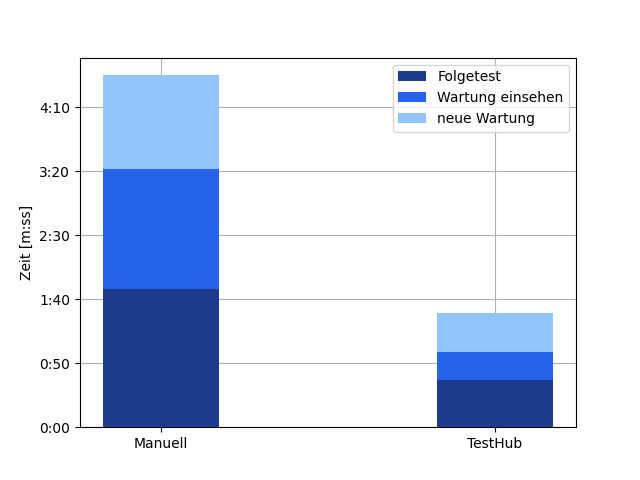
\includegraphics[width=\linewidth]{speedtests/validierung_Zeit.png}
      \caption{Zeitersparnis}
    \end{subfigure}%
    \begin{subfigure}{.5\textwidth}
      \centering
      \includegraphics[width=\linewidth]{speedtests/validierung_cursordistanz.png}
      \caption{Mauszeigerdistanz}
    \end{subfigure}\\
    \begin{subfigure}{.5\textwidth}
        \centering
        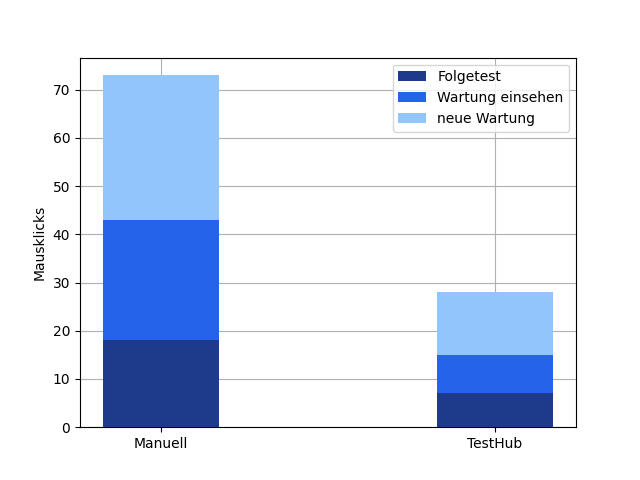
\includegraphics[width=\linewidth]{speedtests/validierung_Mausklicks.png}
        \caption{Mausklicks}
      \end{subfigure}%
      \begin{subfigure}{.5\textwidth}
        \centering
        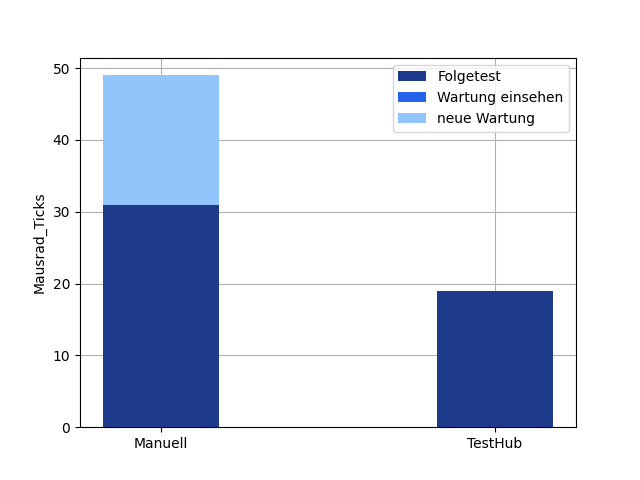
\includegraphics[width=\linewidth]{speedtests/validierung_Mausrad_Ticks.png}
        \caption{Mausrad Ticks}
      \end{subfigure}
    \caption{Ergebnisse der Bedienbarkeitsvalidierung, aufgeschlüsselt nach Aufgaben}
   
\end{figure}

\begin{longtable}{| P{0.15\linewidth} | P{0.15\linewidth} | P{0.15\linewidth} | P{0.15\linewidth} | P{0.15\linewidth} |} 
  \hline
  \textbf{Aufgabe} & \textbf{Zeit} & \textbf{Mauszeiger- distanz} & \textbf{Klickzahl} & \textbf{Mausrad Ticks}\\[0.5ex] 
  \hline
  
  Folgeticket & 65,74\% & 70,13\% & 61,11\% & 38,71\% \\ [0.5ex] \hline
  Wartung einsehen & 76,60\% & 66,68\% & 68,00\% & - \\ [0.5ex] \hline
  neuer Wartungstermin & 58,91\% & -12,46\% & 56,67\% & 100\% \\ [0.5ex] \hline
  \textbf{Gesamt} & 67,64\% & 45,59\% & 61,64\% & 61,22\% \\ [0.5ex] \hline
  \caption{Nach Aufgaben aufgeschlüsselte Verbesserung durch TestHub }\label{tab:valres}
\end{longtable}
\textit{Alle Tests wurden lokal auf einem Dell Latitude 5590 (Intel Core i5-8350U CPU
@ 1.70GHz; 8GB RAM) mit angeschlossenem 32'' Bildschirm mit 4K (3840$\times$2160) Auflösung im HomeOffice durchgeführt}

\newpage

Auf den ersten subjektiven Blick fällt auf, dass TestHub in fast allen Bereichen eine erhebliche
Verbesserung aufweist. Gerade der wichtigste Faktor, der Zeitaufwand, konnte durch TestHub 
mit einer Verbesserung von ca. 70\% erheblich reduziert werden. 
Da in einem maximierten Browserfenster statt im kleinen Windows 
Dateiexplorerfenster gearbeitet wird, ist die Mauszeigerdistanz bei der Erstellung eines neuen 
Wartungstermins etwas größer als bisher. Aufgrund des dennoch geringeren Zeitaufwands
stellt sich dieser Sachverhalt jedoch nicht als nachteilig dar.
Zusätzlich auffallend ist, dass nur beim Folgetest heraussuchen das Mausrad 
benutzt werden muss. Die Benutzung des 
Mausrads beim Erstellen eines neuen Wartungstermins fällt somit komplett weg, was für 
eine Übersichtlichkeit des \gls{UI}s spricht.

Um diese Aussagen zu belegen, müsste jedoch eine viel größere Studie mit mehreren 
Teilnehmern und Testfällen durchgeführt werden.

\newpage


